% Author: Rasmus Pank Roulund
\documentclass{minimal}
\usepackage{tikz}
\usetikzlibrary{calc,trees,positioning,arrows,chains,shapes.geometric,%
    decorations.pathreplacing,decorations.pathmorphing,shapes,%
    matrix,shapes.symbols}

\tikzset{
>=stealth',
  punktchain/.style={
    rectangle, 
    rounded corners, 
    % fill=black!10,
    draw=black, very thick,
    text width=10em, 
    minimum height=3em,
    fill=black!20,
    text centered, 
    on chain},
  line/.style={draw, thick, <-},
  element/.style={
    tape,
    top color=white,
    bottom color=blue!50!black!60!,
    minimum width=8em,
    draw=blue!40!black!90, very thick,
    text width=10em, 
    minimum height=3.5em, 
    text centered, 
    on chain},
  every join/.style={->, thick,shorten >=1pt},
  decoration={brace},
  tuborg/.style={decorate},
  tubnode/.style={midway, right=2pt},
}
\begin{document}
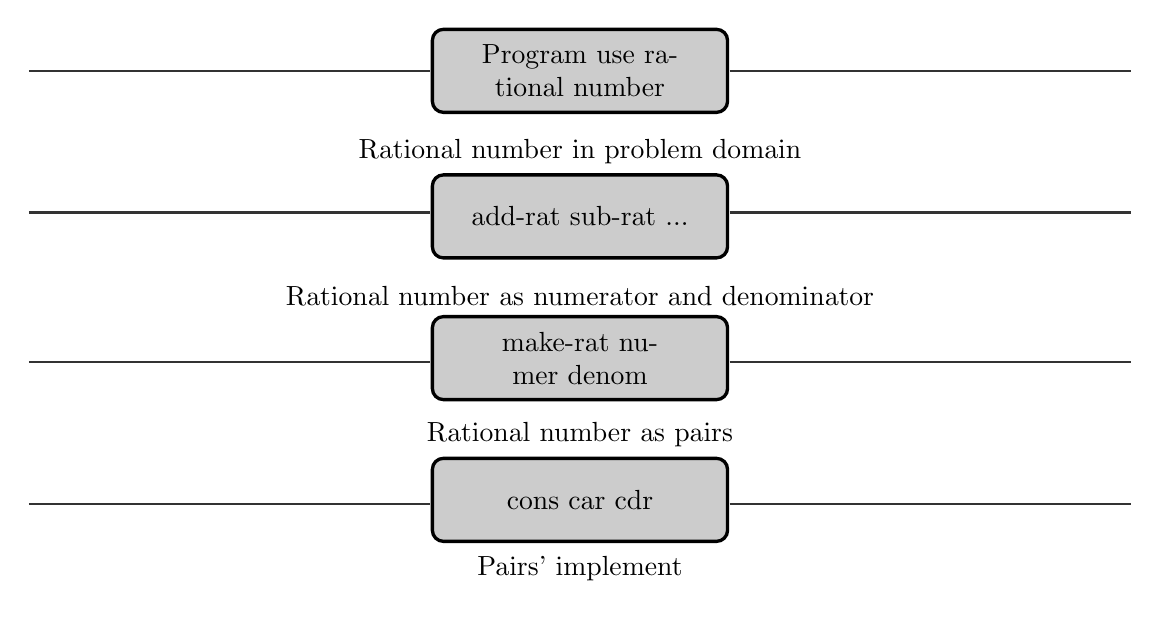
\begin{tikzpicture}
  [node distance=.8cm,
  start chain=going below,]
     \node[punktchain] (rat-procedure) at (3.5,-5.5) {Program use rational number};
     \node[punktchain] (operators) at (3.5,-6.) {add-rat\ sub-rat\ ...};
     \node[punktchain] (constructor) at (3.5,-7.8) {make-rat\ numer\ denom};
     \node[punktchain] (pairs) at (3.5,-9.6) {cons car cdr};
     \draw[-,thick,draw=black!80] (-3.5,-5.5) -- (1.6,-5.5);
     \draw[-,thick,draw=black!80] (5.4,-5.5) -- (10.5,-5.5);
     \draw[-,thick,draw=black!80] (-3.5,-7.3) -- (1.6,-7.3);
     \draw[-,thick,draw=black!80] (5.4,-7.3) -- (10.5,-7.3);
     \draw[-,thick,draw=black!80] (-3.5,-9.2) -- (1.6,-9.2);
     \draw[-,thick,draw=black!80] (5.4,-9.2) -- (10.5,-9.2);
     \draw[-,thick,draw=black!80] (-3.5,-11.) -- (1.6,-11.);
     \draw[-,thick,draw=black!80] (5.4,-11.) -- (10.5,-11.);
     %\draw[tuborg,draw=white!10] ($(-3.5,-4.5)$) -- ($(10.5,-4.5)$) node[above, midway]  {Teori};
     \draw[tuborg,draw=white!10] ($(-3.5,-6.8)$) -- ($(10.5,-6.8)$) node[above, midway]  {Rational number in problem domain};
     \draw[tuborg,draw=white!10] ($(-3.5,-8.6)$) -- ($(10.5,-8.6)$) node[above, midway]  {Rational number as numerator and denominator};
     \draw[tuborg,draw=white!10] ($(-3.5,-10.4)$) -- ($(10.5,-10.4)$) node[above, midway]  {Rational number as pairs};
     \draw[tuborg,draw=white!10] ($(-3.5,-12.1)$) -- ($(10.5,-12.1)$) node[above, midway]  {Pairs'  implement};
  \end{tikzpicture}
\end{document}